%%%%%%%%%%%%%%%%%%%%%%%%%%%%%%%%%%%%%%%%%%%%%%%%%%%%%%%%%%%%%%%%%%%%%%%%%%%%


\documentclass[draft]{agujournal2019}
\usepackage{url} 
%\usepackage{lineno}
%\usepackage[inline]{trackchanges} %for better track changes. finalnew option will compile document with changes incorporated.
\usepackage{soul}
\usepackage{lscape}
\usepackage{adjustbox}
\usepackage{float}
\usepackage{amsmath}
\usepackage{amssymb}
\usepackage{amsthm}
\usepackage{physics}
\usepackage{setspace}
\usepackage{fix-cm}
\usepackage{booktabs}


\usepackage{graphicx}

\usepackage{wrapfig}
\usepackage{blindtext}
%Table-related commands
\usepackage{array}
%\setlength{\arrayrulewidth}{1mm}
%\setlength{\tabcolsep}{18pt}
%\renewcommand{\arraystretch}{1.5}
%\newcolumntype{s}{>{\columncolor[HTML]{AAACED}} p{3cm}}
% %-------------------------------------------------------


% defined commands
\newcommand{\unit}[1]{\ensuremath{\, \mathrm{#1}}}
% "Colored Marker" commands: wrap text in, e.g., \red{...} to highlight that color
\newcommand{\red}[1]{\textcolor{red}{#1}}
\newcommand{\blue}[1]{\textcolor{blue}{#1}}
\newcommand{\purple}[1]{\textcolor{purple}{#1}}
\newcommand{\avg}[1]{\left\langle #1 \right\rangle}
\newcommand{\vel}[0]{\mathbf{u}}
\newcommand{\B}[0]{\mathbf{B}}

%uncomment this for single-spaced version
\draftfalse

\begin{document}
\SetSinglespace{}
% preliminary title
\title{PHYS 6268: Nonlinear Dynamics: Problem Set 1}

% I defaulted to alphabetical last name, no preference here
\authors{C. Michael Haynes\affil{1}}

\affiliation{1}{School of Earth and Atmospheric Sciences, Georgia Institute of Technology, Atlanta GA, USA}


\section*{Strogatz Book: Problems 2.5.3, 2.6.1, 2.7.3, 2.7.4, \& 2.8.3}


\section{Problem 2.5.3}
\label{sec:p1}



\textbf{Consider the equation $\dot x = rx + x^3$, where $r>0$ is fixed. Show that $x(t)\longrightarrow\pm\infty$ in finite time, starting from any initial condition $x_0$.}
\par

The equation 
\begin{equation}
    \label{eqn:p1}
    \dot x = rx + x^3 \qquad r\in\mathbb{R}^+
\end{equation}
is separable, yielding an approach to solve for the trajectories $x(t)$ of the system analytically. The constant $r>0$ forces there to exist only a single root, $x^*=0$. Since $\mathrm{sgn}(x) = \mathrm{sgn}(x^3)$, one can see by inspection that the sign of $\dot x(t=0)\equiv\dot x_0$ is the same as the sign of the initial condition $x_0$. For positive $x_0$, $\dot x_0 >0$, and $x(t)$ grows from $x_0$. The same is true for negative initial conditions. As time increases, trajectories that start with a positive $x_0$ only ever increase, and negative trajectories only continue to decrease. Thus, for any values of $x_0\neq0$, the absolute value of the trajectory is only amplified in positive $t$ due to the sign of the derivative being the same as the sign of $x(t)$. We can see by inspection that the derivative diverges with $x^3$ as time increases. Since solutions to $\dot x = x(t)$ increase with $e^t$, this relationship $\dot x \propto x^3$ represents a super-exponential increase in $|x|$ as $t$ increases, which reaches infinity in finite time.
\par
However, to show more rigorously that this divergence occurs in finite time, we seek the solutions to equation (\ref{eqn:p1}) via separation:
\begin{equation*}
    \frac{\mathrm{d}x}{x(r+x^2)} = {\mathrm{d}t} \qquad .
\end{equation*}
This can be directly integrated using partial fraction decomposition: 
\begin{equation*}
    \implies t = \int_{x_0}^{x(t)} \frac{\mathrm{d}x}{x(r+x^2)} = \int_{x_0}^{x(t)} \mathrm{d}x \, \left(\frac{A}{x} + \frac{Bx+C}{r+x^2} \right) \qquad ,
\end{equation*}
which yields the following expression for the real constants ($A,B,\&\,C$):
\begin{equation*}
    A(r + x^2) + Bx^2 + C = 1 = Ar + Cx + (A+B)x^2 \qquad .
\end{equation*}
This constraint is a polynomial in $x$, immediately requiring that $A+B=0$ and that $A\,r=1$. Hence, we have:
\begin{align*}
    A = \frac{1}{r} \\
    B = - \frac{1}{r} \\ 
    C = 0
\end{align*}
From which our integrand becomes
\begin{equation*}
    t = \int_{x_0}^{x(t)} \mathrm{d}x \, \left(\frac{1}{rx} - \frac{x}{r(r+x^2)} \right) \qquad .
\end{equation*}
Integrating yields (suppressing the $(t)$ for each instance of $x$) the following:
\begin{equation*}
    \frac{1}{r} \ln{|x|} - \frac{1}{2r} \ln{|r+x^2|} - \left(\frac{1}{r} \ln{|x_0|} - \frac{1}{2r} \ln{|r+x_0^2|}\right) = t \qquad .
\end{equation*}
We collapse the constants into an additional one 
\begin{equation*}
    \bar{c}_1/r \equiv \frac{1}{r} \ln{|x_0|} - \frac{1}{2r} \ln{|r+x_0^2|} = \frac{1}{r} \ln{\left|\frac{x_0}{\sqrt{r+x_0^2}}\right|}
\end{equation*}
for simplicity and convenience of manipulation. Combining the natural logarithms and rearranging the expression yields
\begin{equation*}
    \ln{\left|\frac{x}{\sqrt{x^2+r}}\right|} = rt + \bar c_1 \qquad .
\end{equation*}
Exponentiation yields 
\begin{equation*}
    \left|\frac{x}{\sqrt{x^2+r}}\right|=\exp(rt+\bar c_1) \implies \frac{x^2}{x^2+r}=\exp(2rt+2\bar c_1) 
\end{equation*}
It should be noted with the treatment of the absolute value and squares that we are neglecting any complex solutions of $x(t)$, and considering only the real branches. With the redefinition of $\bar c_2 \equiv e^{2\bar c_1} $, we are left with 
\begin{equation*}
    \frac{x^2(t)}{x^2(t)+r} = \bar c_2 e^{2rt} \qquad .
\end{equation*}
Algebraic manipulations yields the solution for $x^2(t)$:
\begin{equation}
    \label{eqn:p1_soln}
    x^2(t) = \frac{r \bar c_2 e^{2rt}}{1 - \bar c_2 e^{2rt}} \implies x(t) = \pm \frac{r\bar c_2 e^{rt}}{\sqrt{1 - \bar c_2 e^{2rt}}} \qquad \mathrm{where} \qquad \bar c_2 = \left(\frac{x_0^2}{r+x_0^2}\right) \quad .
\end{equation}
Hence, depending on the sign of $x_0$ (explained above), the solution will diverge either to positive or negative infinity with increasing $t$. 
\par
Since we have solved equation (\ref{eqn:p1}) analytically, we can see that $x(t)$ diverges to $\pm\infty$ for finite $t$, specifically at the critical point $t_c$ when 
\begin{equation*}
    1-\bar c_2 e^{2rt} = 0 \implies t_c = \frac{1}{2r} \ln{\left(\frac{1}{\bar c_2}\right)} \qquad .
\end{equation*}


\par
We note that this can be solved more quickly (and probably more elegantly) with a comparison to solutions of $\dot x = x^3$, since $|rx + x^3| > |x^3| \quad  \forall x\in\{\mathbb{R}/\{x^*=0\}\}$.

% \subsection{Part (b)}
% \label{subsec:p1a}

% \textbf{Using your physical intuition, explain why it now becomes obvious that $x^*=0$ is an unstable fixed point and $x^*=\pi$ is stable.}
% \par






\section{Problem 2.6.1}
\label{sec:p2}



\textbf{Explain this paradox: a simple harmonic oscillator $m \ddot x = -kx$ is a system that oscillates in one dimension (along the $x$-axis). However, the text says one-dimensional systems cannot oscillate.}
\par

This discrepancy is because the simple harmonic oscillator described exists in one \emph{spatial} dimension, but the trajectories actually specify unique coordinates in phase space: that is, both a position $x$ and a \emph{velocity} $\dot x$ are required to specify the system. The one-dimensional, second order system described in this problem is equivalent to a two-dimensional, first order system. This equivalence is what allows such a system to oscillate: for a system described by $\dot x = f(x)$, there cannot be oscillations because the system cannot ``turn around" under such a law. In contrast, this turning around is mediated by the changing velocity prescribed from the simple harmonic motion. In other words, the notion that one-dimensional systems cannot oscillate is generally true if the system is of the form $\dot x = f(x)$, but not the form $\ddot x = f(x)$.




\section{Problem 2.7.3}
\label{sec:p3}



\textbf{For the vector field $\dot x = \sin{x}$, plot the potential function $V(x)$ and identify all the equilibrium points and their stability.}
\par

The potential function for a dynamical system governed by $\dot x = f(x)$ is defined via 
\begin{equation*}
    f(x) = -\frac{\mathrm{d}V}{\mathrm{d}x} \qquad .
\end{equation*}
Equilibrium points are given by values of $V(x)$ where $\frac{\mathrm{d}V}{\mathrm{d}x} = 0$, or rather, fixed points of the vector field. Otherwise, $V(x)$ decreases along trajectories as time increases (i.e., trajectories move towards lower potential). 
\par
The vector field we consider is $\dot x = \sin{x}$. The potential function $V(x)$ is calculated via
\begin{equation*}
    \frac{\mathrm{d}V}{\mathrm{d}x} = -\sin{x} \implies \int \,\mathrm{d}V = \int (-\sin{x})\mathrm\,{\mathrm{d}}x \qquad ,
\end{equation*}
which yields:
\begin{equation*}
    V(x) = \cos{x} \qquad .
\end{equation*}
Then, equilibrium points of the vector field correspond to (for $k\in\mathbb{N}$):
\begin{equation}
\label{eqn:p3}
\begin{array}{cc}
  \frac{\mathrm{d}V}{\mathrm{d}x}=0 \longrightarrow \Bigg\{ & 
    \begin{array}{cc}
      \mathrm{stable:}\,\, (2k+1)\pi\\
      \mathrm{unstable:}\,\, 2k\pi \\
    \end{array}
\end{array}
\end{equation}
The solution for the potential $V$ (as well as the system $f$ for reference) are shown in Figure \ref{fig:p3_potential}. 
\begin{figure}
    \hspace*{-0.7cm}
    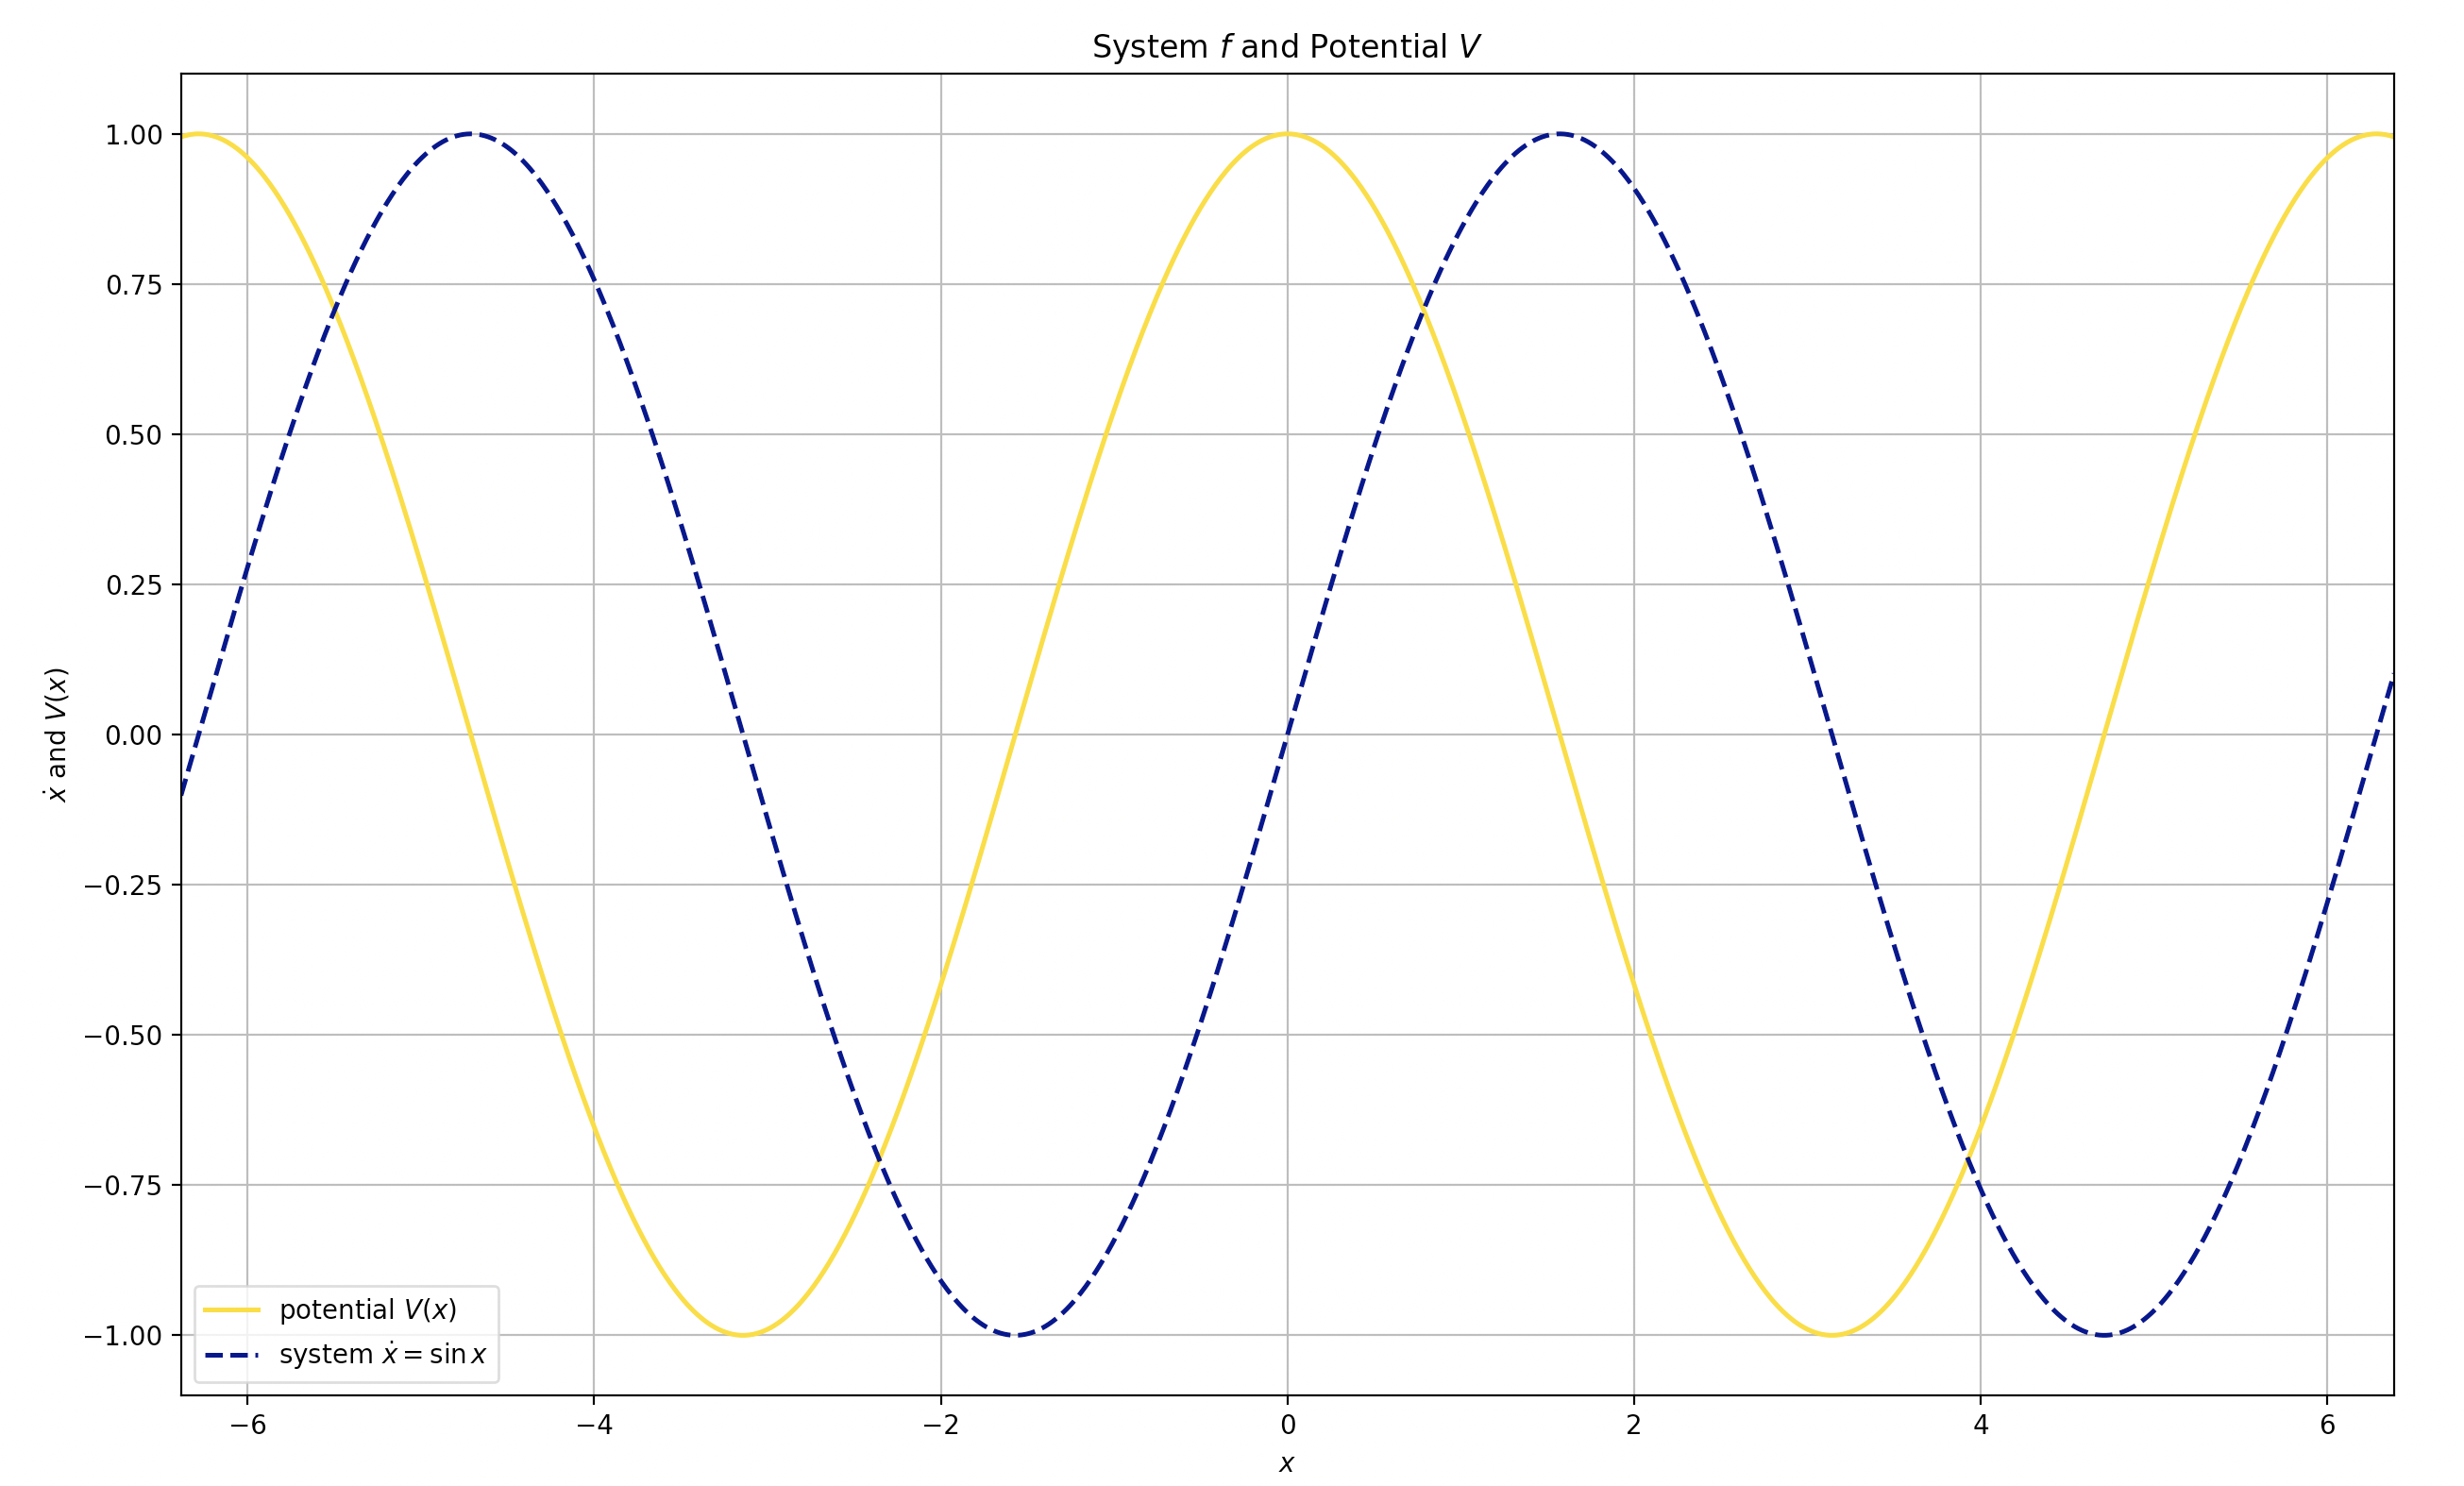
\includegraphics[width=1.1\linewidth]{figs/p3.png}
    \caption{Potential function $V(x)$ (solid gold) and the corresponding dynamical system $\dot x = f(x) = \sin{x}$ (dashed navy) are shown. The functions both continue to $x=\pm\infty$ with periods of $2\pi$. }
    \label{fig:p3_potential}
\end{figure}



\section{Problem 2.7.4}
\label{sec:p4}



\textbf{For the vector field $\dot x = 2+\sin{x}$, plot the potential function $V(x)$ and identify all the equilibrium points and their stability.}
\par
Following the approach of problem (\ref{sec:p3}), we calculate the potential 
\begin{equation*}
    \frac{\mathrm{d}V}{\mathrm{d}x} = -(2+\sin{x}) \implies \int \,\mathrm{d}V = \int -(2+\sin{x})\mathrm\,{\mathrm{d}}x \qquad ,
\end{equation*}
and completing the integration, we find that the potential $V$ is given by
\begin{equation*}
    V(x) = \cos{x} - 2 x \qquad .
\end{equation*}
This system has \emph{no} fixed points: the derivative $\dot x = f(x)=2+\sin{x}$ satisfies $\dot x(t) > 0 \,\,\forall t\in\mathbb{R}$, so the trajectories $x(t)$ are always increasing regardless of the initial data at $x(t=0)$.
\par
The solution for the potential (as well as the system $f$ for reference) are shown in Figure \ref{fig:p4_potential}. It is clear from the potential ($V(x)$, gold curve) how the trajectories continue to flow infinitely, since there are no local minima even with the continuous inflection from the trigonometric term. Hence, the system always diverges.
\begin{figure}
    \hspace*{-0.7cm}
    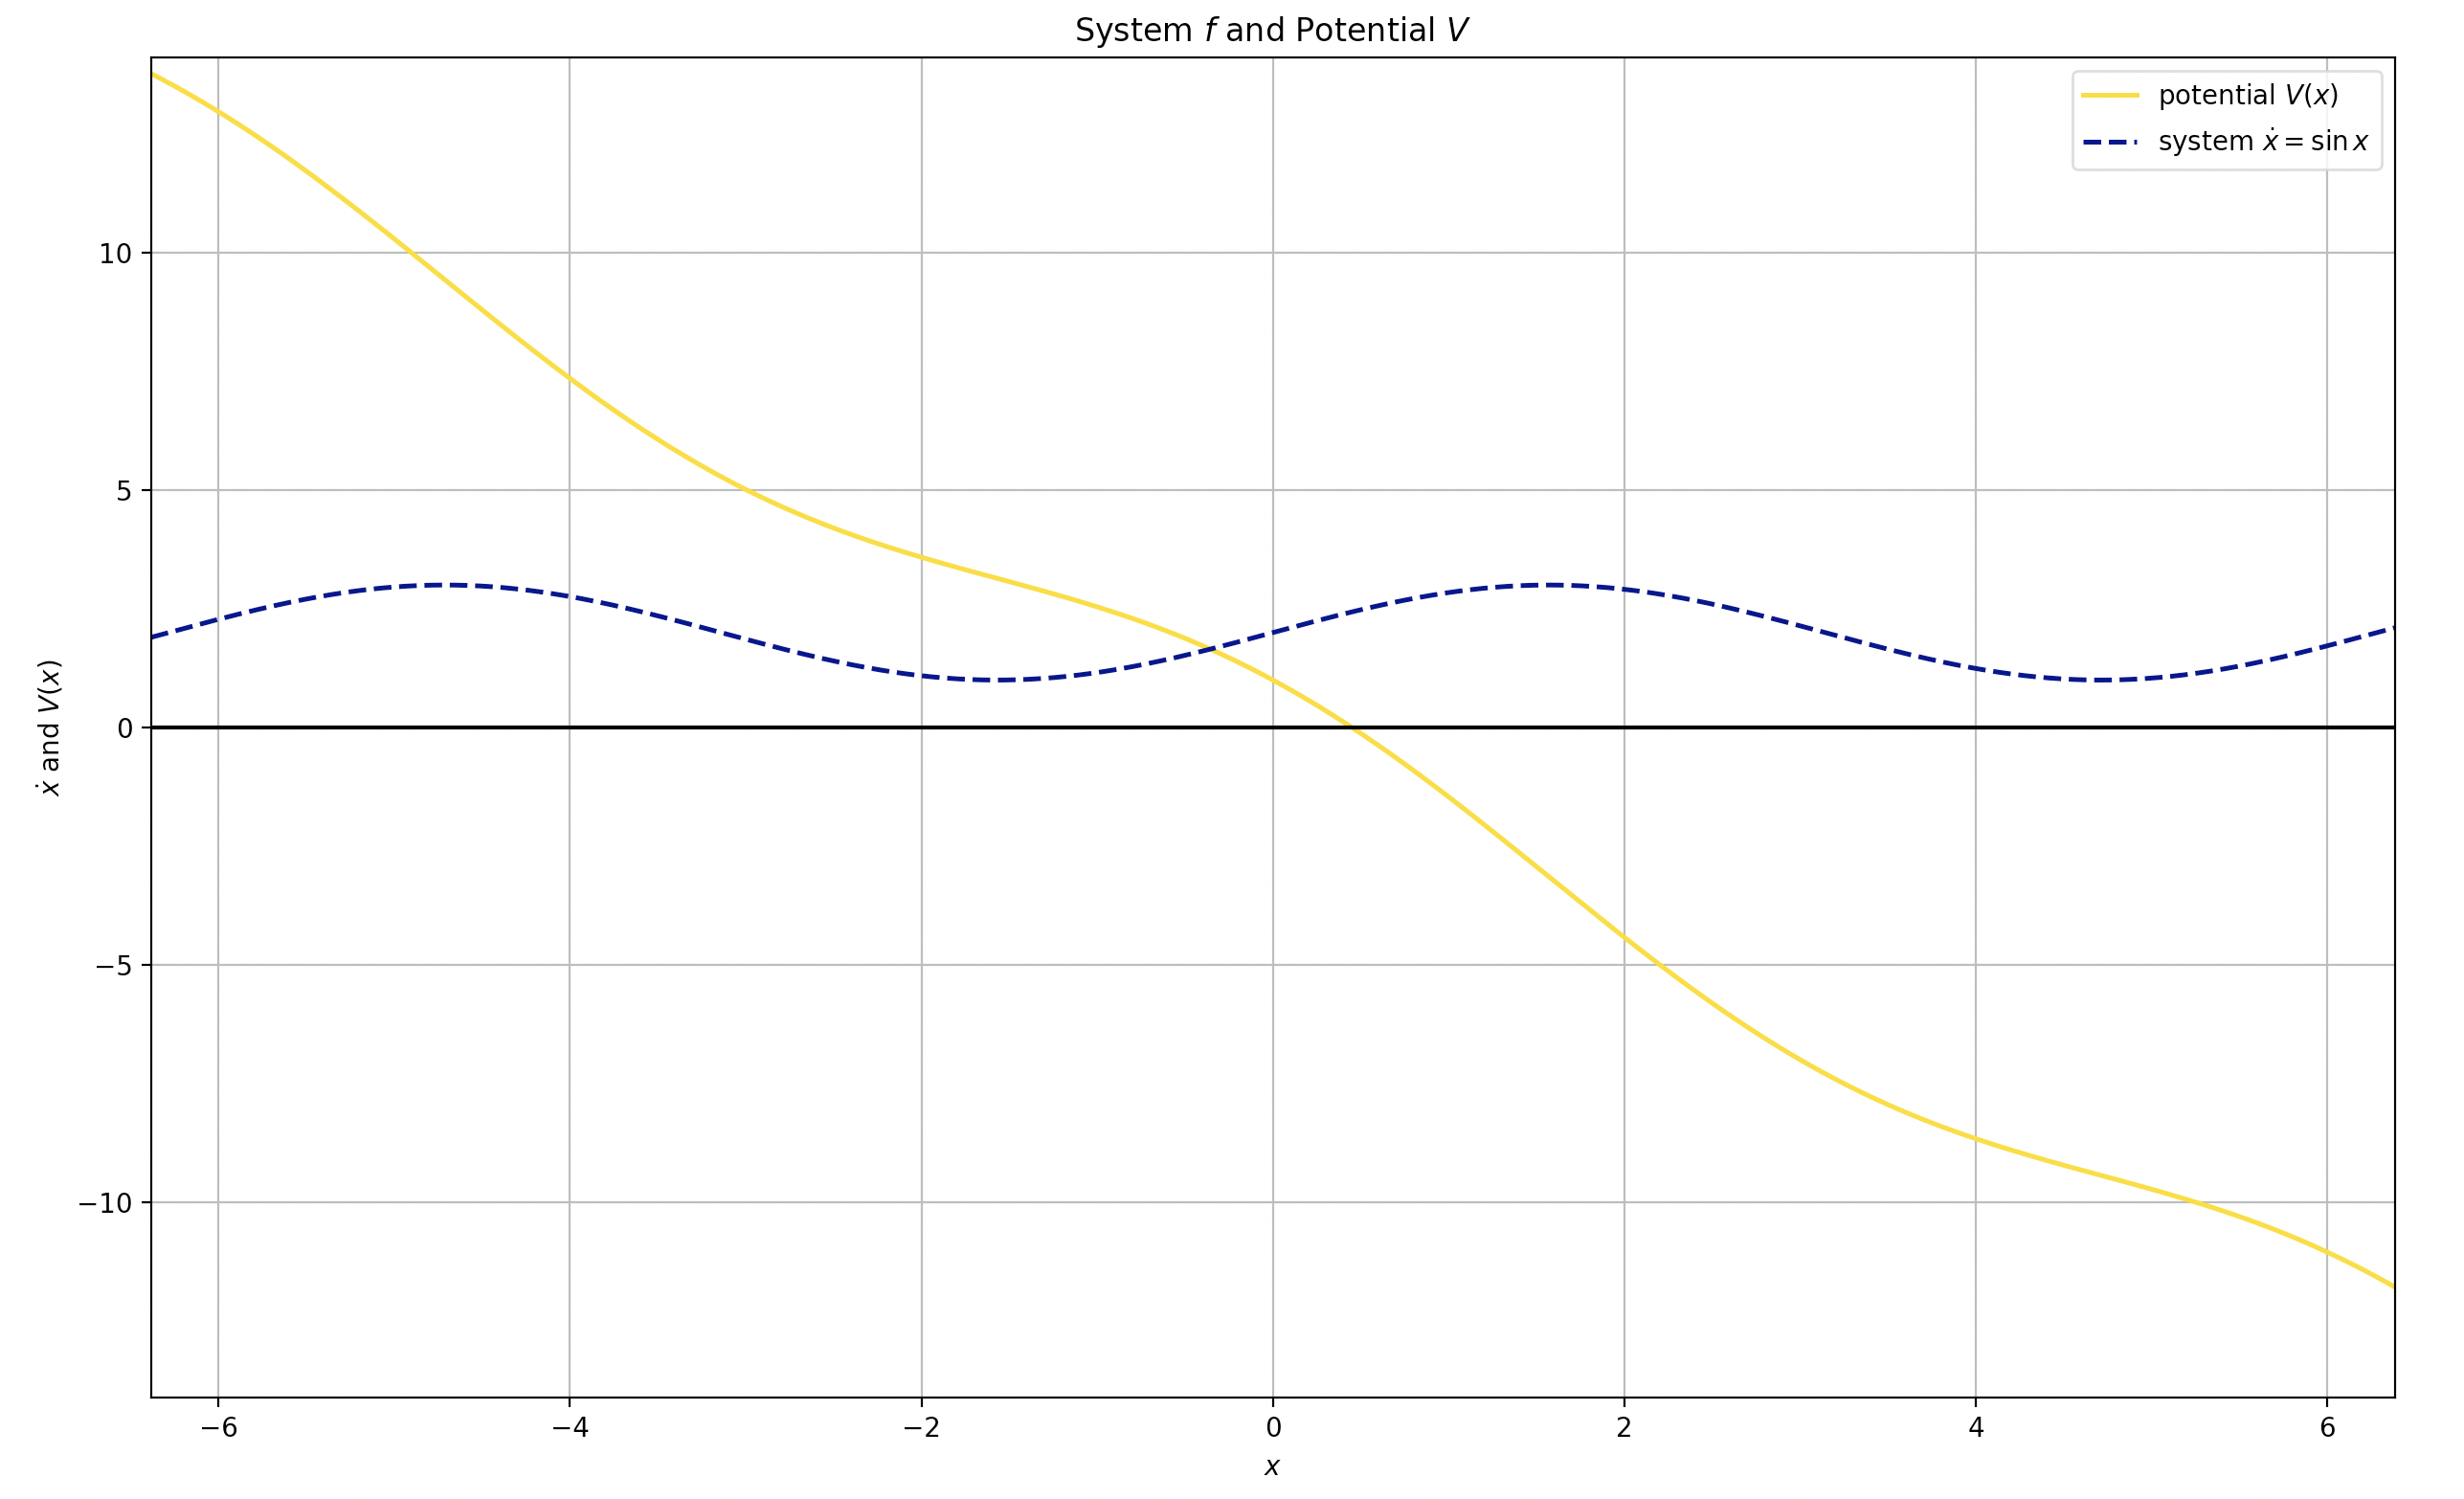
\includegraphics[width=1.1\linewidth]{figs/p4.png}
    \caption{Potential function $V(x)$ (solid gold) and the corresponding dynamical system $\dot x = f(x) = 2+\sin{x}$ (dashed navy) are shown. The functions both continue to $x=\pm\infty$ with periods of $2\pi$. }
    \label{fig:p4_potential}
\end{figure}




\newpage
\section{Problem 2.8.3}
\label{sec:p5}



\textbf{(Calibrating the Euler Method).}
\par


\subsection{Part (a)}
\label{subsec:p5a}
\textbf{Solve the initial value problem $\dot x = -x,\,\,x(t=0)=1$ analytically. What is the exact value of $x(1)$?}

Let $x(t=0) \equiv x_0 = 1$. The analytical solution to the initial value problem is obtained via direct integration:
\begin{equation*}
    \int_{x_0}^{x(t)} \,\frac{\mathrm{d}x}{x} = - \int_0^t \, \mathrm{d}t \qquad .
\end{equation*}
Which becomes 
\begin{equation*}
    \implies e^{\ln{\left|\frac{x(t)}{x_0}\right|}} = e^{-t} \qquad ,
\end{equation*}
\begin{equation*}
    \implies x(t) = x_0 e^{-t} = e^{-t} \qquad \implies x(t=1) = e^{-1} = \frac{1}{e} \approx 0.367879441
\end{equation*}


\subsection{Part (b)}
\label{subsec:p5b}
\textbf{Using the Euler method with a step size of $\Delta t = 10^{-n}$ for $n\in\{0,1,2,3,4\}$, estimate $x(1)$ numerically. Call the result $\hat{x}(1)$.}

The values of each estimate are tabulated below. The error ranges from $E=1-1/e\approx0.632$ at step $n=0$ to $E=1.8\cdot10^{-5}$ with a timestep given by $n=4$. 

\begin{table}
    \centering
    \begin{tabular}{cc}
    \toprule % Top rule from booktabs package
        \textbf{$n\longrightarrow\Delta t=10^{-n}$} & \textbf{Estimate $\hat{x}(1)$} \\
        \midrule % Middle rule from booktabs package
        0 & 1.000000\\
        1 & 0.348678\\
        2 & 0.369729\\
        3 & 0.368063\\
        4 & 0.367861\\
        \bottomrule
    \end{tabular}
    \caption{Estimates $\hat{x}(1)$ for the system in section \ref{subsec:p5a}. }
    \label{tab:p5b}
\end{table}


\subsection{Part (b)}
\label{subsec:p5b}
\textbf{Plot the error $E=|\hat{x}(1)-x(1)|$ as a function of $\Delta t$. Then plot $\ln{E}$ vs. $\ln{\Delta t}$. Explain the results. }
The plots are included in Figures \ref{fig:p5ci} and \ref{fig:p5cii}. 
\par
Figure \ref{fig:p5ci} demonstrates how the error drops linearly. The linear rate changes slightly, however, moving from the zeroth order method to the first order method. This is likely because the zeroth order method still completed one timestep, so the difference between one and ten timesteps will be slightly different than the difference between 10 and 100. 
\par
Figure \ref{fig:p5cii} depicts how this is only a slight change in the ``improvement" between successive timestep jumps; the log/log plot of this Figure illustrates more ``evenly" the picture of the increasingly small timestep. Since Euler's method is a first order method, the accuracy increases linearly with decreasing timestep. The method being accurate to first order implies that the error is a function of $(\Delta t)^2$.



\begin{figure}[t]
    % \hspace*{-0.7cm}
    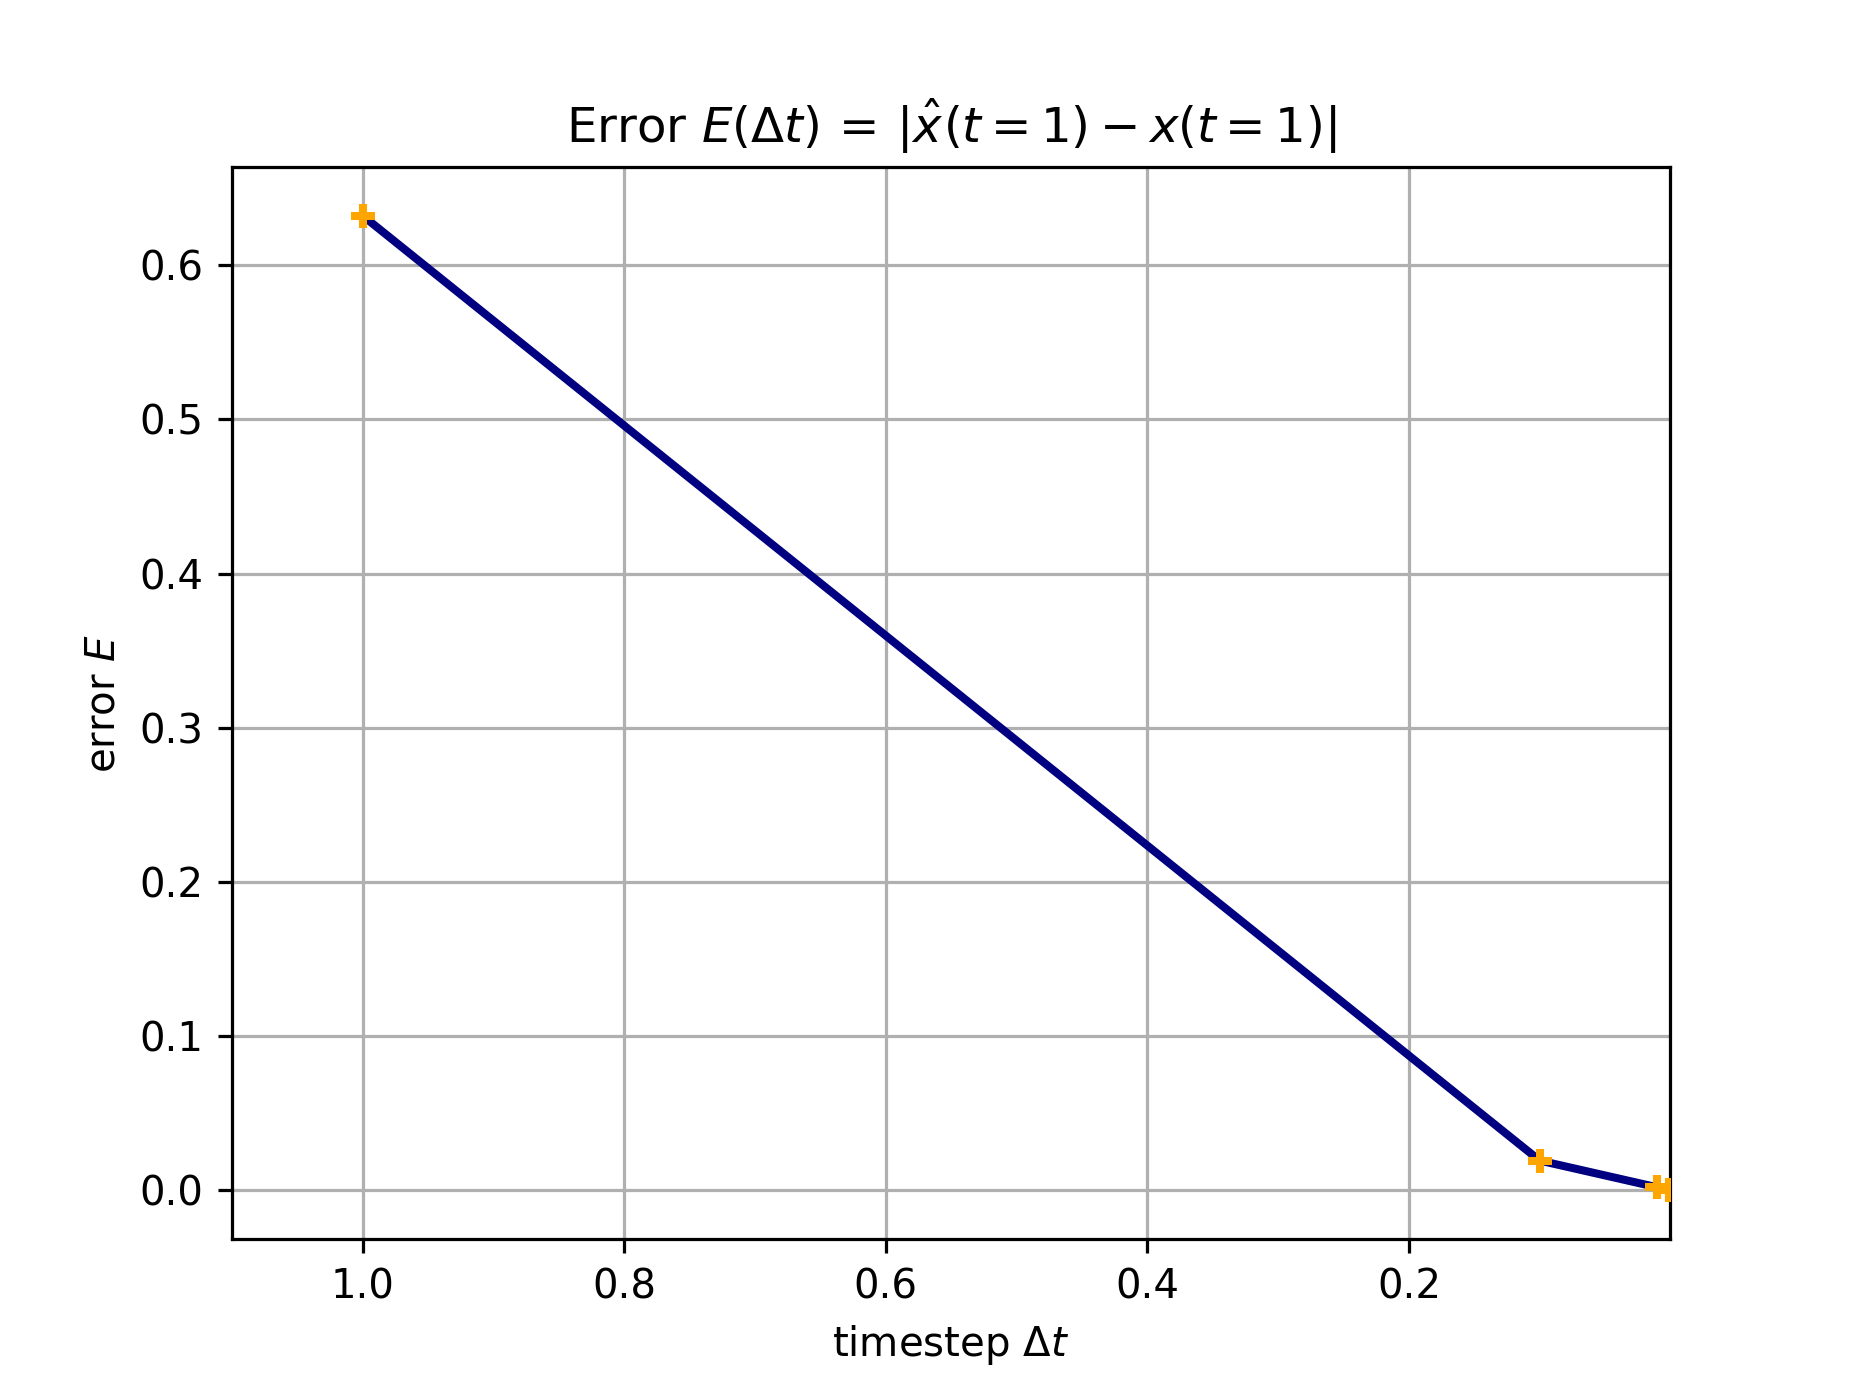
\includegraphics[width=0.91\linewidth]{figs/figure2.8.3.c.i.png}
    \centering
    \caption{Error $E(\Delta t) = |\hat{x}(1)-x(1)|$ plotted as a function of the timestep $\Delta t$. The plot is shown on a linear scale. }
    \label{fig:p5ci}
\end{figure}




\begin{figure}[b]
    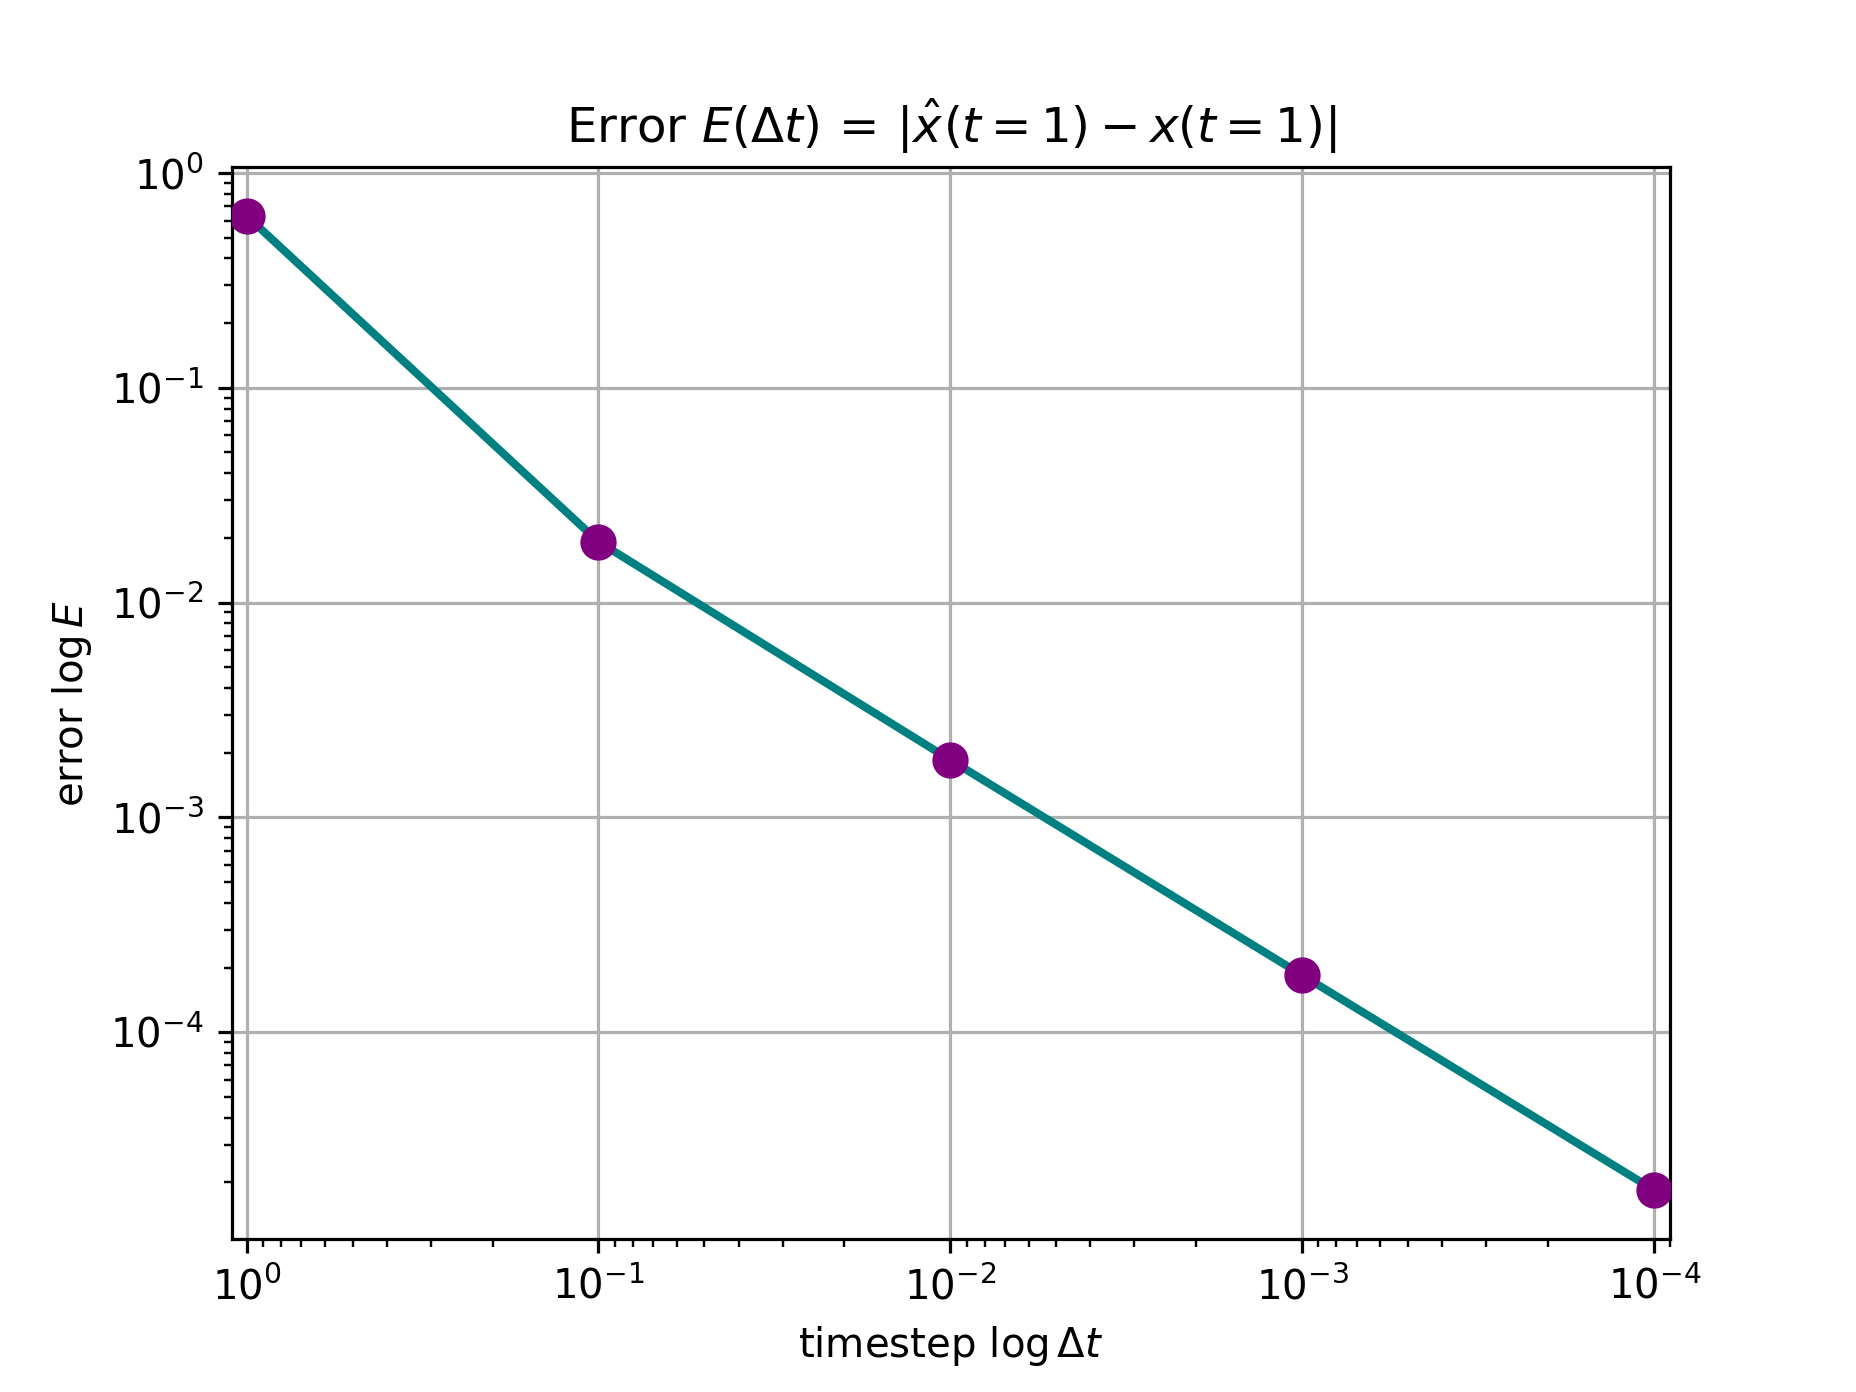
\includegraphics[width=.91\linewidth]{figs/figure2.8.3.c.ii.png}
    \centering
    \caption{The Error ($E(\Delta t) = |\hat{x}(1)-x(1)|$) plotted against $(\Delta t)$ on a log-log scale. }
    \label{fig:p5cii}
\end{figure}
Figure \ref{fig:p5cii-2} shows the contents of Figure \ref{fig:p5cii}, however, this is done in exactly the way Strogatz asked for it, plotting $\log{E}$ versus $\log{\Delta t}$.

\begin{figure}[b]
    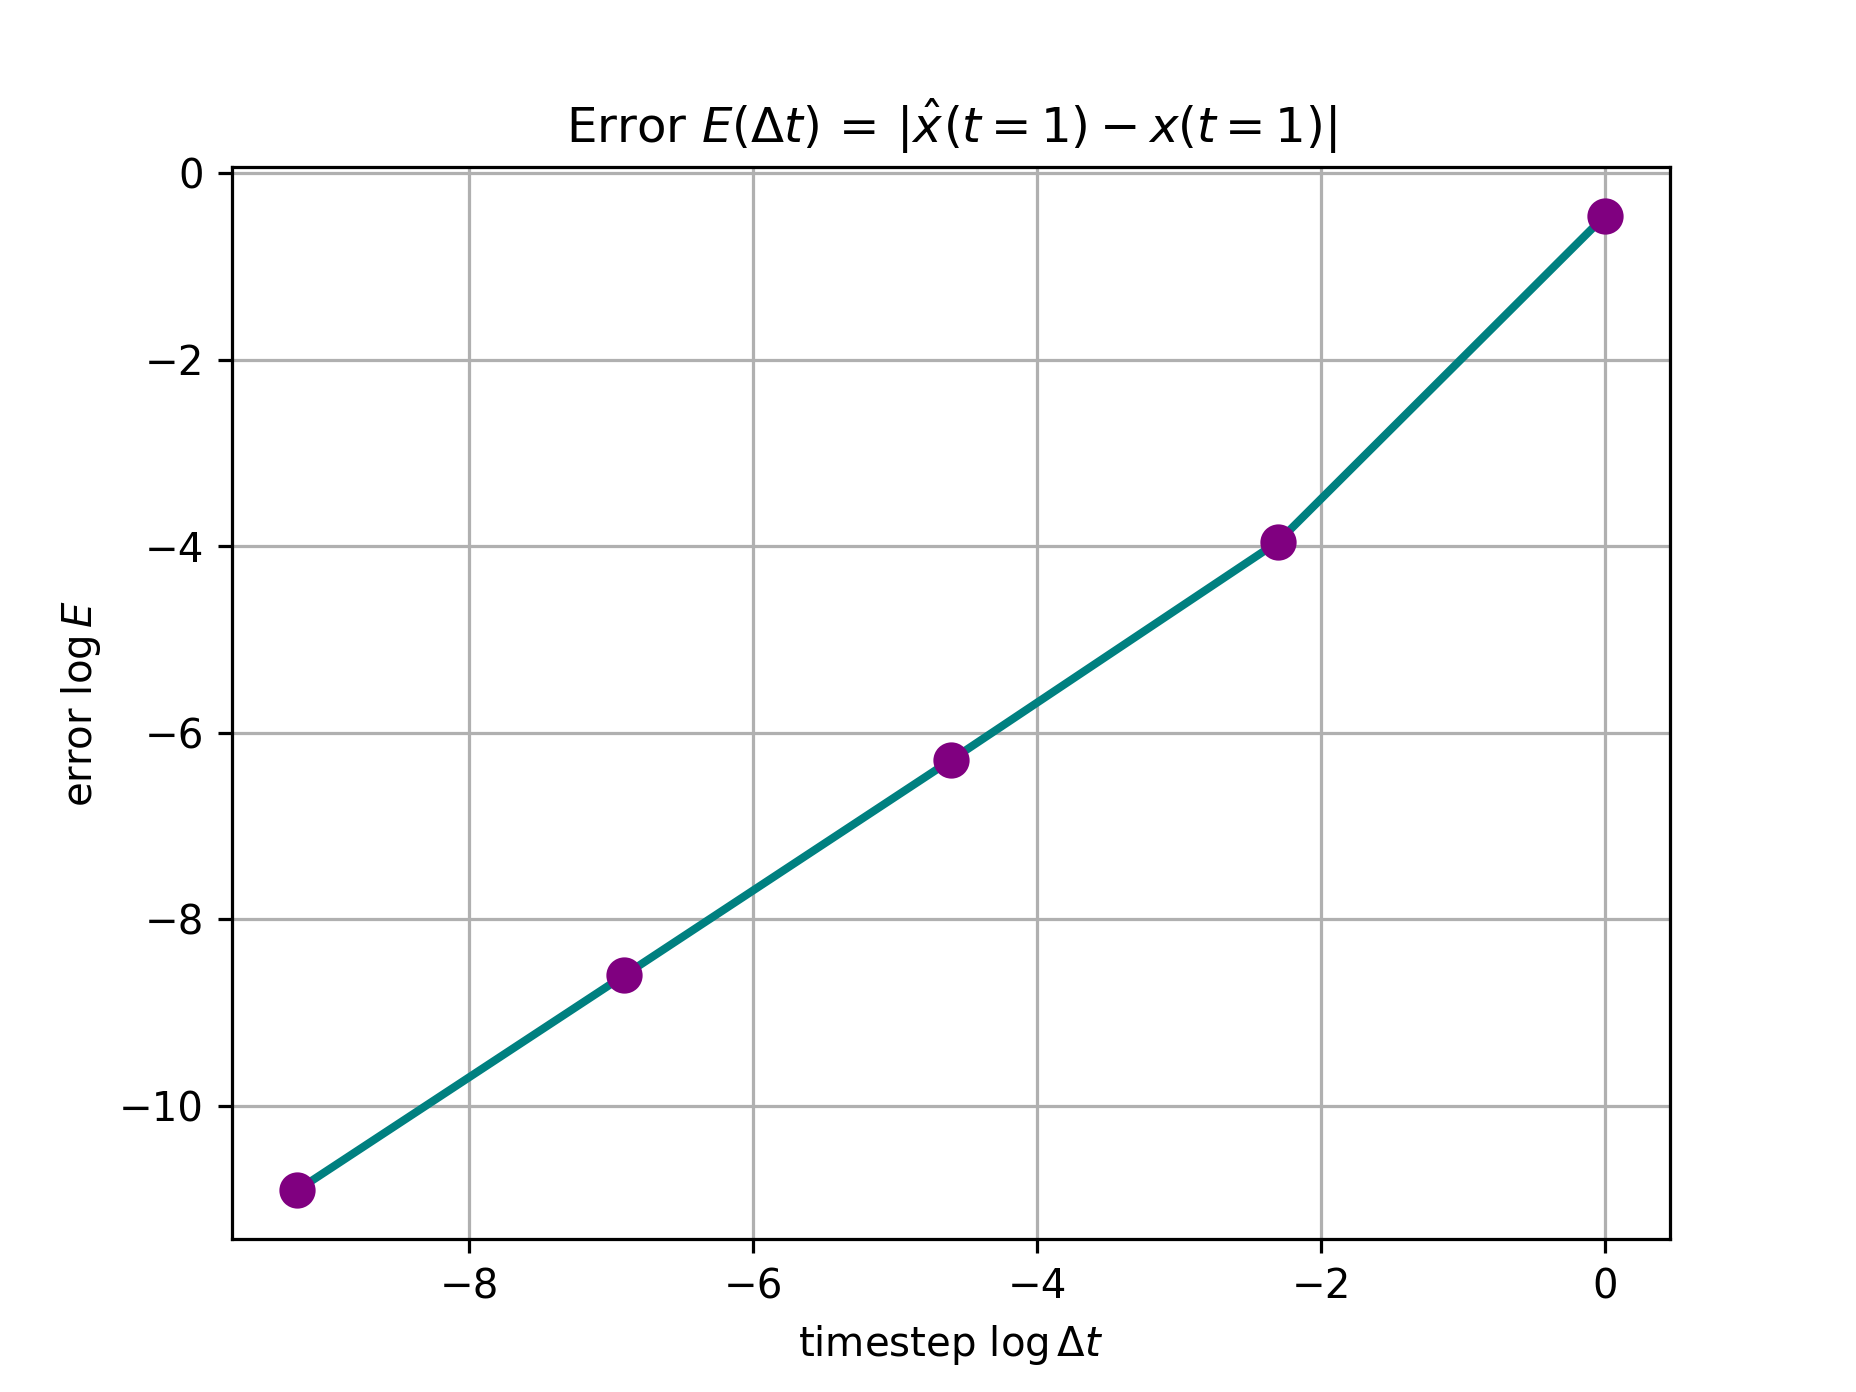
\includegraphics[width=.91\linewidth]{figs/figure2.8.3.c.ii-2.png}
    \centering
    \caption{The logarithm of the Error ($\ln{E}(\Delta t) = \ln|\hat{x}(1)-x(1)|$) plotted as a function of timestep $(\Delta t)$. }
    \label{fig:p5cii-2}
\end{figure}


\clearpage
\section{Software Usage}
The entirety of the work was carried out on pen and paper prior to typesetting, except for that of section \ref{sec:p5} and the plotting: this was completed using python (\verb|numpy| and \verb|matplotlib|). 

%\section{Acknowledgments}
\newpage














%%%%%%%%%%%%%%%%%%%%%%%%%%%%%%%%%%%%%%%%%%%%%%%
% \newpage
% \clearpage

%\bibliography{MHD}
\end{document}
